\documentclass[aspectratio=169]{beamer}
\usepackage[T1]{fontenc}
\usepackage[utf8]{inputenc}
\usepackage{lmodern}
\usepackage{microtype}
\usepackage{xcolor}
\usepackage{tikz}
\usetikzlibrary{positioning, arrows.meta, calc}
\usepackage{fontawesome5}

\definecolor{wurgreen}{HTML}{34B233}
\definecolor{darkgreen}{HTML}{1F6B1E}
\definecolor{darknavy}{HTML}{1A1A2E}
\definecolor{midgray}{HTML}{6B7280}
\definecolor{lightgray}{HTML}{F3F4F6}
\definecolor{lightgreen}{HTML}{E8F7E8}
\definecolor{bodytext}{HTML}{1F2937}
\definecolor{warnred}{HTML}{FEE2E2}
\definecolor{warnborder}{HTML}{EF4444}

\usetheme{default}
\usecolortheme{default}
\usefonttheme{professionalfonts}
\setbeamertemplate{navigation symbols}{}
\setbeamertemplate{itemize items}{\textcolor{wurgreen}{\textbullet}}
\setbeamertemplate{itemize subitem}{\textcolor{midgray}{--}}
\setbeamercolor{frametitle}{fg=white, bg=darknavy}
\setbeamerfont{frametitle}{size=\large, series=\bfseries}
\setbeamertemplate{frametitle}{%
  \begin{beamercolorbox}[wd=\paperwidth, ht=1.1cm, dp=0.2cm, leftskip=0.6cm]{frametitle}
    \usebeamerfont{frametitle}\insertframetitle
  \end{beamercolorbox}}
\setbeamercolor{background canvas}{bg=white}
\setbeamercolor{normal text}{fg=bodytext}
\setbeamertemplate{footline}{%
  \begin{beamercolorbox}[wd=\paperwidth, ht=0.4cm, dp=0.15cm]{footline}
    \hspace{0.5cm}\textcolor{midgray}{\tiny Bags, Vectors \& Transformers · Wageningen University \& Research}%
    \hfill\textcolor{midgray}{\tiny \insertframenumber}\hspace{0.4cm}
  \end{beamercolorbox}}

\begin{document}

% ── TITLE ──────────────────────────────────────────────────────────────────
{
\setbeamertemplate{footline}{}
\begin{frame}[plain]
  \begin{tikzpicture}[remember picture, overlay]
    \fill[darknavy] (current page.south west) rectangle (current page.north east);
    \fill[wurgreen] (current page.south west) rectangle
      ([xshift=0.45cm]current page.north west);
    \node[anchor=west, text=white, font=\huge\bfseries, text width=13cm]
      at ([xshift=1.1cm, yshift=1.2cm]current page.west)
      {Bags, Vectors \& Transformers};
    \node[anchor=west, text=wurgreen, font=\large, text width=12cm]
      at ([xshift=1.1cm, yshift=0.05cm]current page.west)
      {Ethics, Open Models \& Distillation · Day 4, Part 2};
    \node[anchor=west, text=midgray, font=\small, text width=12cm]
      at ([xshift=1.1cm, yshift=-1.5cm]current page.west)
      {Denise J. Roth, PhD Candidate\\
       Strategic Communication Group · Wageningen University \& Research};
  \end{tikzpicture}
\end{frame}
}

% ── SLIDE 1: the turn ─────────────────────────────────────────────────────
\begin{frame}{The Questions That Matter Most}
\vspace{0.2cm}
{\small LLMs are powerful and easy to use. That is exactly why we need to slow down and ask
the \textbf{harder questions} --- especially as researchers, where our choices have
consequences for reproducibility, ethics, and trust.}

\medskip
\begin{itemize}\setlength\itemsep{8pt}
  \item[\textcolor{wurgreen}{\faBalanceScale}]
    What are the \textbf{ethical and practical risks} of using LLMs in research?
  \item[\textcolor{wurgreen}{\faLockOpen}]
    Why do \textbf{open-weight} and \textbf{local} models matter so much?
  \item[\textcolor{wurgreen}{\faMagic}]
    How can \textbf{distillation} give us the best of both worlds?
\end{itemize}

\medskip
{\small\textcolor{midgray}{\textit{This is where a thoughtful researcher separates themselves
from someone just calling an API.}}}
\end{frame}

% ── SLIDE 2: ethical/practical risks ──────────────────────────────────────
\begin{frame}{Risks You Need to Take Seriously}
\vspace{0.2cm}
\begin{columns}[T]
  \column{0.48\textwidth}
  \vspace{0pt}
  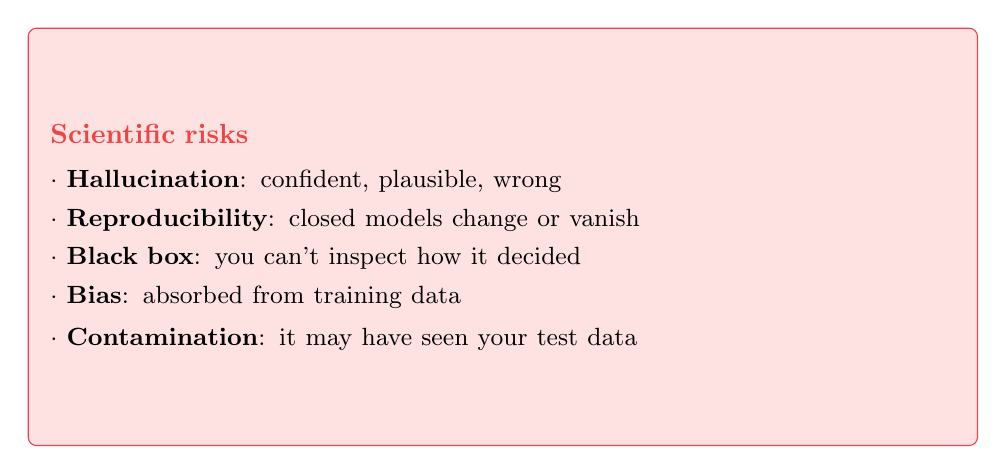
\begin{tikzpicture}
    \node[fill=warnred, draw=warnborder, rounded corners=3pt,
          inner xsep=8pt, inner ysep=8pt, text width=\columnwidth-18pt, minimum height=5.3cm]{%
      \textcolor{warnborder}{\textbf{Scientific risks}}\\[5pt]
      {\small
      $\cdot$ \textbf{Hallucination}: confident, plausible, wrong\\[3pt]
      $\cdot$ \textbf{Reproducibility}: closed models change or vanish\\[3pt]
      $\cdot$ \textbf{Black box}: you can't inspect how it decided\\[3pt]
      $\cdot$ \textbf{Bias}: absorbed from training data\\[3pt]
      $\cdot$ \textbf{Contamination}: it may have seen your test data}};
  \end{tikzpicture}

  \column{0.48\textwidth}
  \vspace{0pt}
  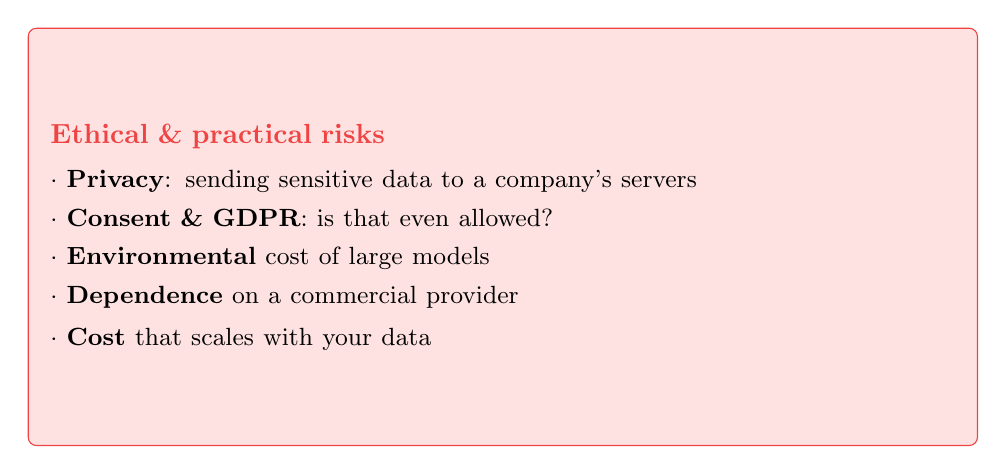
\begin{tikzpicture}
    \node[fill=warnred, draw=warnborder, rounded corners=3pt,
          inner xsep=8pt, inner ysep=8pt, text width=\columnwidth-18pt, minimum height=5.3cm]{%
      \textcolor{warnborder}{\textbf{Ethical \& practical risks}}\\[5pt]
      {\small
      $\cdot$ \textbf{Privacy}: sending sensitive data to a company's servers\\[3pt]
      $\cdot$ \textbf{Consent \& GDPR}: is that even allowed?\\[3pt]
      $\cdot$ \textbf{Environmental} cost of large models\\[3pt]
      $\cdot$ \textbf{Dependence} on a commercial provider\\[3pt]
      $\cdot$ \textbf{Cost} that scales with your data}};
  \end{tikzpicture}
\end{columns}
\end{frame}

% ── SLIDE 3: responsible use principles ───────────────────────────────────
\begin{frame}{Principles for Responsible Use}
\vspace{0.3cm}
\begin{columns}[T]
  \column{0.48\textwidth}
  \vspace{0pt}
  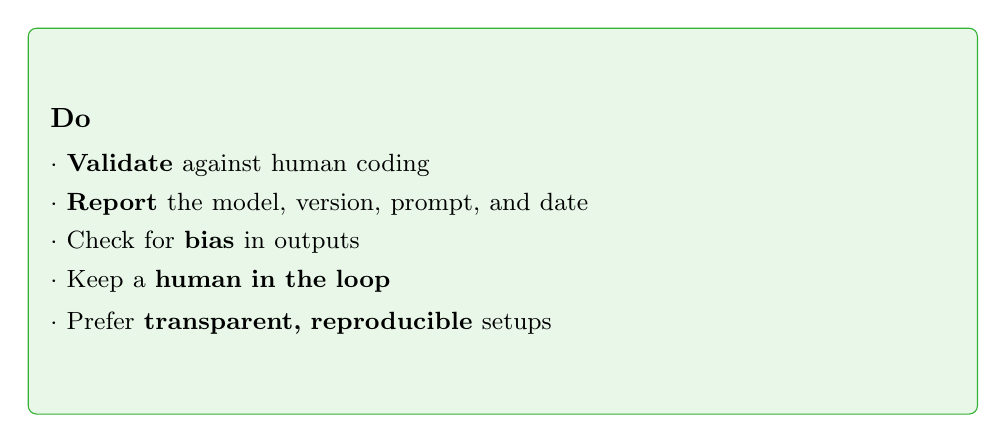
\begin{tikzpicture}
    \node[fill=lightgreen, draw=wurgreen, rounded corners=3pt,
          inner xsep=8pt, inner ysep=8pt, text width=\columnwidth-18pt, minimum height=4.9cm]{%
      \textbf{Do}\\[5pt]
      {\small
      $\cdot$ \textbf{Validate} against human coding\\[3pt]
      $\cdot$ \textbf{Report} the model, version, prompt, and date\\[3pt]
      $\cdot$ Check for \textbf{bias} in outputs\\[3pt]
      $\cdot$ Keep a \textbf{human in the loop}\\[3pt]
      $\cdot$ Prefer \textbf{transparent, reproducible} setups}};
  \end{tikzpicture}

  \column{0.48\textwidth}
  \vspace{0pt}
  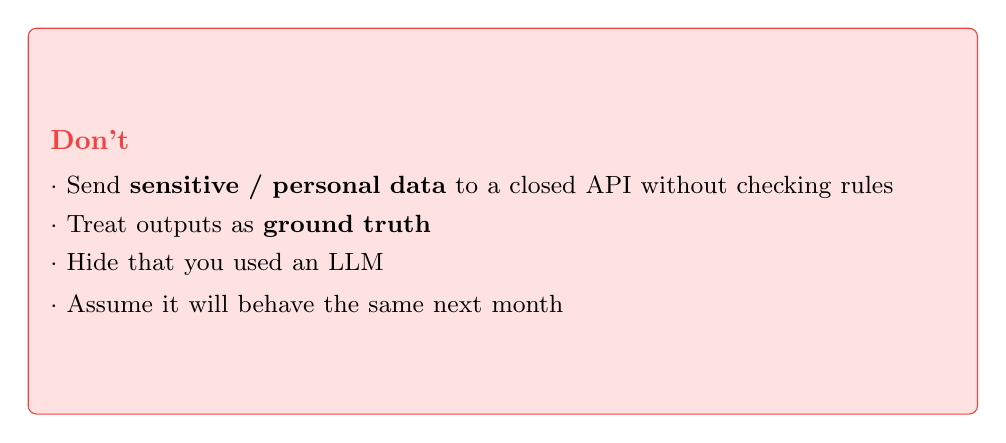
\begin{tikzpicture}
    \node[fill=warnred, draw=warnborder, rounded corners=3pt,
          inner xsep=8pt, inner ysep=8pt, text width=\columnwidth-18pt, minimum height=4.9cm]{%
      \textcolor{warnborder}{\textbf{Don't}}\\[5pt]
      {\small
      $\cdot$ Send \textbf{sensitive / personal data} to a closed API without checking rules\\[3pt]
      $\cdot$ Treat outputs as \textbf{ground truth}\\[3pt]
      $\cdot$ Hide that you used an LLM\\[3pt]
      $\cdot$ Assume it will behave the same next month}};
  \end{tikzpicture}
\end{columns}

\medskip
{\small\textcolor{midgray}{\textit{Transparency is the throughline: another researcher should be
able to understand and, ideally, reproduce exactly what you did.}}}
\end{frame}

% ── SLIDE 4: closed vs open ───────────────────────────────────────────────
\begin{frame}{Closed vs.\ Open-Weight Models}
\vspace{0.2cm}
{\small A crucial distinction. \textbf{Closed} models (GPT-4, Claude, Gemini) live behind an
API. \textbf{Open-weight} models (Llama, Mistral, Qwen, Gemma) can be \textbf{downloaded and
run yourself}.}

\medskip
\begin{columns}[T]
  \column{0.48\textwidth}
  \vspace{0pt}
  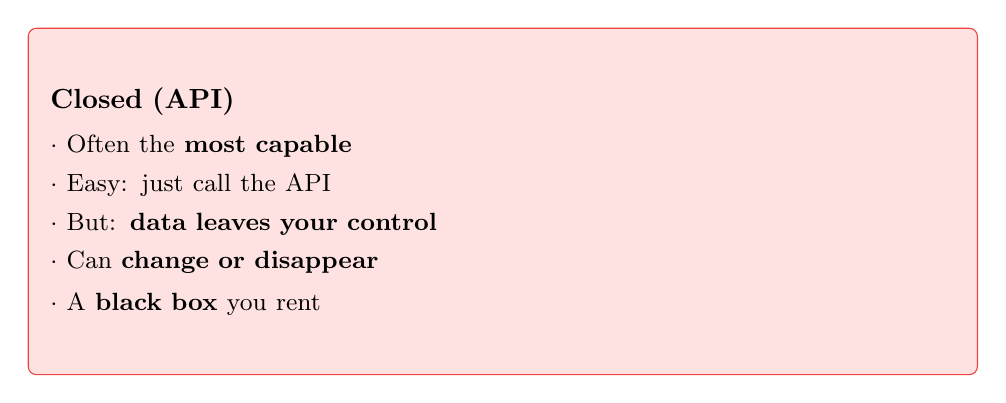
\begin{tikzpicture}
    \node[fill=warnred, draw=warnborder, rounded corners=3pt,
          inner xsep=8pt, inner ysep=8pt, text width=\columnwidth-18pt, minimum height=4.4cm]{%
      \textbf{Closed (API)}\\[5pt]
      {\small
      $\cdot$ Often the \textbf{most capable}\\[3pt]
      $\cdot$ Easy: just call the API\\[3pt]
      $\cdot$ But: \textbf{data leaves your control}\\[3pt]
      $\cdot$ Can \textbf{change or disappear}\\[3pt]
      $\cdot$ A \textbf{black box} you rent}};
  \end{tikzpicture}

  \column{0.48\textwidth}
  \vspace{0pt}
  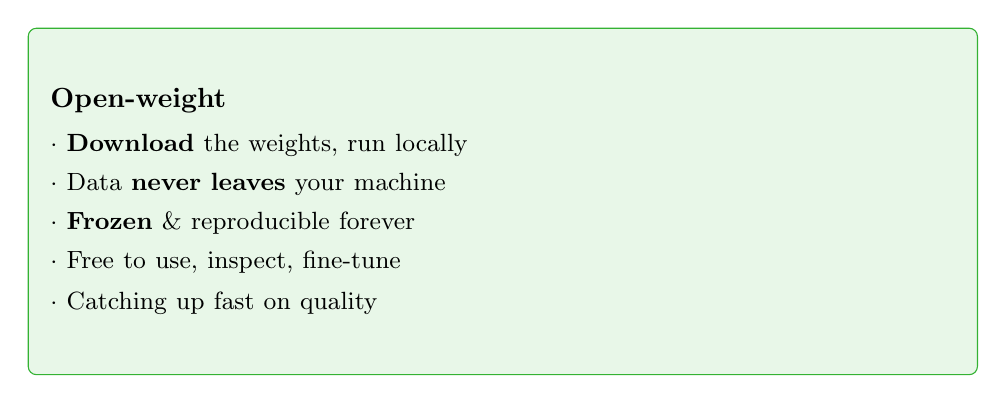
\begin{tikzpicture}
    \node[fill=lightgreen, draw=wurgreen, rounded corners=3pt,
          inner xsep=8pt, inner ysep=8pt, text width=\columnwidth-18pt, minimum height=4.4cm]{%
      \textbf{Open-weight}\\[5pt]
      {\small
      $\cdot$ \textbf{Download} the weights, run locally\\[3pt]
      $\cdot$ Data \textbf{never leaves} your machine\\[3pt]
      $\cdot$ \textbf{Frozen} \& reproducible forever\\[3pt]
      $\cdot$ Free to use, inspect, fine-tune\\[3pt]
      $\cdot$ Catching up fast on quality}};
  \end{tikzpicture}
\end{columns}
\end{frame}

% ── SLIDE 5: the case for open + local ────────────────────────────────────
\begin{frame}{The Case for Open \& Local Models}
\vspace{0.2cm}
{\small For \textbf{research}, open-weight models you run locally are often the
\emph{better} choice --- not despite being less flashy, but because of what they give you:}

\medskip
\begin{columns}[T]
  \column{0.48\textwidth}
  \vspace{0pt}
  {\small
  \textcolor{wurgreen}{\faShieldAlt}\enspace \textbf{Privacy \& GDPR}\\
  {\footnotesize Sensitive data (interviews, patient text) never leaves your control.}\\[7pt]
  \textcolor{wurgreen}{\faRedo}\enspace \textbf{Reproducibility}\\
  {\footnotesize The exact model is frozen --- your study can be rerun in five years.}\\[7pt]
  \textcolor{wurgreen}{\faSearchPlus}\enspace \textbf{Transparency}\\
  {\footnotesize You can inspect, document, and share exactly what you used.}}

  \column{0.48\textwidth}
  \vspace{0pt}
  {\small
  \textcolor{wurgreen}{\faEuroSign}\enspace \textbf{Cost}\\
  {\footnotesize No per-call fees --- run it as much as you like on your data.}\\[7pt]
  \textcolor{wurgreen}{\faUnlock}\enspace \textbf{Independence}\\
  {\footnotesize No lock-in to a company that may change terms or prices.}\\[7pt]
  \textcolor{wurgreen}{\faWrench}\enspace \textbf{Control}\\
  {\footnotesize Fine-tune it, adapt it, make it \emph{yours}.}}
\end{columns}

\medskip
{\small\textcolor{midgray}{\textit{Modern open models run on a single GPU --- or even a good
laptop --- with tools like Ollama. The barrier is lower than most people think.}}}
\end{frame}

% ── SLIDE 6: but they are not always the answer ───────────────────────────
\begin{frame}{An Honest Caveat}
\vspace{0.3cm}
{\small Open \& local is not \emph{always} the answer. Being fair about the trade-offs:}

\medskip
\begin{columns}[T]
  \column{0.48\textwidth}
  \vspace{0pt}
  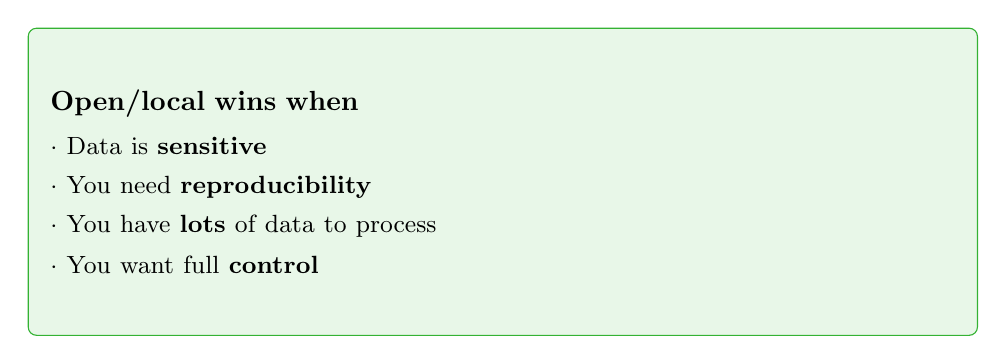
\begin{tikzpicture}
    \node[fill=lightgreen, draw=wurgreen, rounded corners=3pt,
          inner xsep=8pt, inner ysep=8pt, text width=\columnwidth-18pt, minimum height=3.9cm]{%
      \textbf{Open/local wins when}\\[5pt]
      {\small
      $\cdot$ Data is \textbf{sensitive}\\[3pt]
      $\cdot$ You need \textbf{reproducibility}\\[3pt]
      $\cdot$ You have \textbf{lots} of data to process\\[3pt]
      $\cdot$ You want full \textbf{control}}};
  \end{tikzpicture}

  \column{0.48\textwidth}
  \vspace{0pt}
  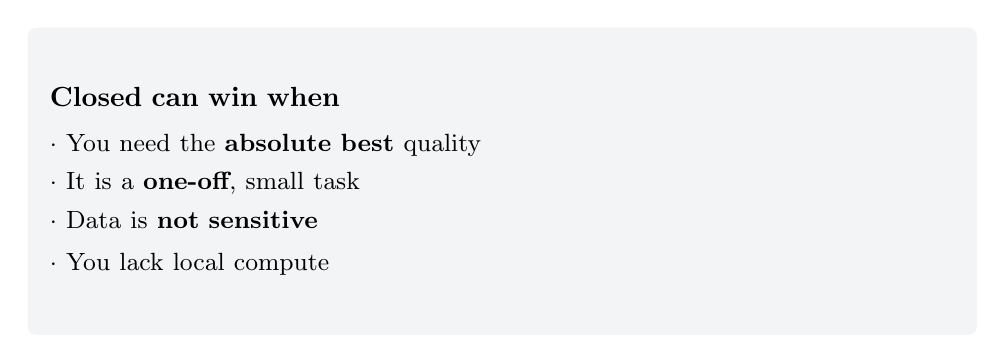
\begin{tikzpicture}
    \node[fill=lightgray, rounded corners=3pt,
          inner xsep=8pt, inner ysep=8pt, text width=\columnwidth-18pt, minimum height=3.9cm]{%
      \textbf{Closed can win when}\\[5pt]
      {\small
      $\cdot$ You need the \textbf{absolute best} quality\\[3pt]
      $\cdot$ It is a \textbf{one-off}, small task\\[3pt]
      $\cdot$ Data is \textbf{not sensitive}\\[3pt]
      $\cdot$ You lack local compute}};
  \end{tikzpicture}
\end{columns}

\medskip
{\small\textcolor{midgray}{\textit{The point is to \textbf{choose deliberately} --- not to
default to a commercial API just because it's the first thing you saw.}}}
\end{frame}

% ── SLIDE 7: distillation - the idea ──────────────────────────────────────
\begin{frame}{Distillation: The Best of Both Worlds}
\vspace{0.2cm}
{\small Here is the elegant idea that ties this whole course together. You do \textbf{not} have
to choose between a powerful-but-expensive LLM and a small-but-cheap BERT. \textbf{Use both.}}

\medskip
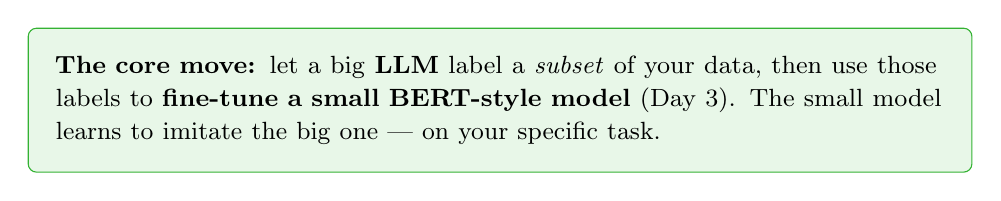
\begin{tikzpicture}
  \node[fill=lightgreen, draw=wurgreen, rounded corners=3pt,
        inner xsep=10pt, inner ysep=10pt, text width=\textwidth-24pt]{%
    {\small \textbf{The core move:} let a big \textbf{LLM} label a \emph{subset} of your data,
    then use those labels to \textbf{fine-tune a small BERT-style model} (Day 3). The small
    model learns to imitate the big one --- on your specific task.}};
\end{tikzpicture}

\medskip
{\small This is a form of \textbf{knowledge distillation}: transferring what a large ``teacher''
model knows into a small, efficient ``student'' model. The student is cheap, fast, local,
reproducible --- and often nearly as good \emph{on your task}.}
\end{frame}

% ── SLIDE 8: distillation - the workflow ──────────────────────────────────
\begin{frame}{The Distillation Workflow}
\vspace{0.4cm}
\begin{center}
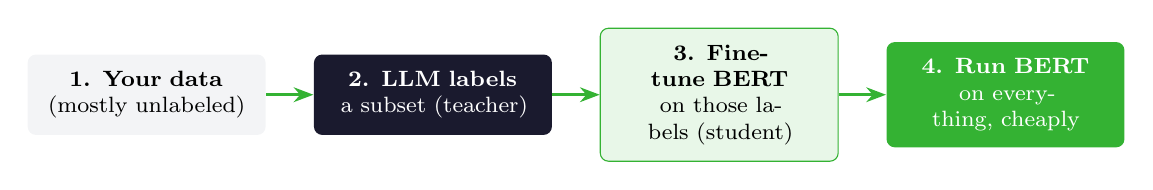
\begin{tikzpicture}[font=\footnotesize, node distance=0.55cm]
  \node[fill=lightgray, rounded corners=3pt, inner sep=6pt, text width=2.6cm, align=center] (data)
    {\textbf{1. Your data}\\ (mostly unlabeled)};
  \node[fill=darknavy, rounded corners=3pt, inner sep=6pt, text width=2.6cm, align=center,
        right=0.6cm of data] (llm)
    {\textcolor{white}{\textbf{2. LLM labels}}\\ \textcolor{white}{a subset (teacher)}};
  \node[fill=lightgreen, draw=wurgreen, rounded corners=3pt, inner sep=6pt, text width=2.6cm,
        align=center, right=0.6cm of llm] (bert)
    {\textbf{3. Fine-tune BERT}\\ on those labels (student)};
  \node[fill=wurgreen, rounded corners=3pt, inner sep=6pt, text width=2.6cm, align=center,
        right=0.6cm of bert] (deploy)
    {\textcolor{white}{\textbf{4. Run BERT}}\\ \textcolor{white}{on everything, cheaply}};
  \draw[-{Stealth[length=2.5mm]}, wurgreen, line width=1pt] (data) -- (llm);
  \draw[-{Stealth[length=2.5mm]}, wurgreen, line width=1pt] (llm) -- (bert);
  \draw[-{Stealth[length=2.5mm]}, wurgreen, line width=1pt] (bert) -- (deploy);
\end{tikzpicture}
\end{center}

\medskip
{\small You pay the LLM cost \textbf{once}, for a subset. The resulting BERT model then labels
your \textbf{entire} corpus --- and every future corpus --- for almost nothing, on your own
machine.}
\end{frame}

% ── SLIDE 9: distillation - why it's great ────────────────────────────────
\begin{frame}{Why Distillation Is So Attractive for Research}
\vspace{0.3cm}
\begin{columns}[T]
  \column{0.48\textwidth}
  \vspace{0pt}
  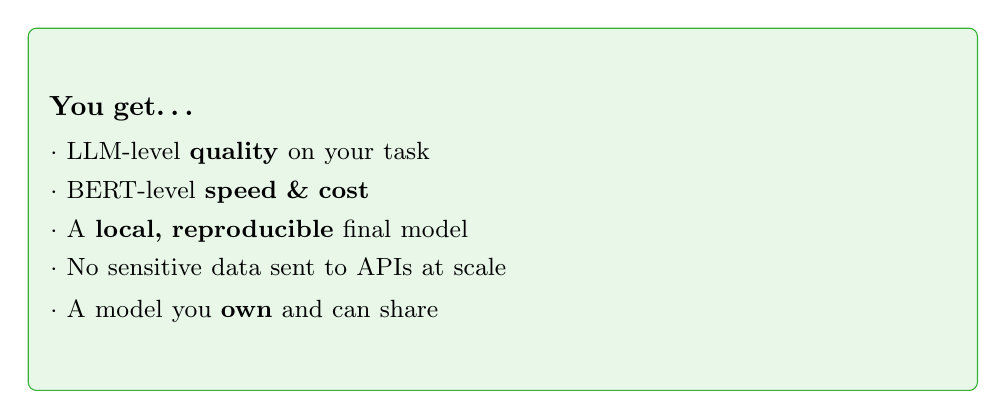
\begin{tikzpicture}
    \node[fill=lightgreen, draw=wurgreen, rounded corners=3pt,
          inner xsep=8pt, inner ysep=8pt, text width=\columnwidth-18pt, minimum height=4.6cm]{%
      \textbf{You get\ldots}\\[5pt]
      {\small
      $\cdot$ LLM-level \textbf{quality} on your task\\[3pt]
      $\cdot$ BERT-level \textbf{speed \& cost}\\[3pt]
      $\cdot$ A \textbf{local, reproducible} final model\\[3pt]
      $\cdot$ No sensitive data sent to APIs at scale\\[3pt]
      $\cdot$ A model you \textbf{own} and can share}};
  \end{tikzpicture}

  \column{0.48\textwidth}
  \vspace{0pt}
  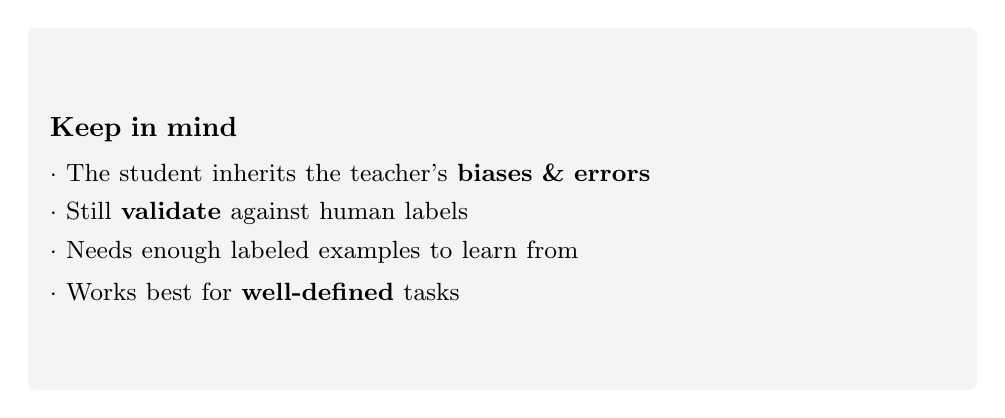
\begin{tikzpicture}
    \node[fill=lightgray, rounded corners=3pt,
          inner xsep=8pt, inner ysep=8pt, text width=\columnwidth-18pt, minimum height=4.6cm]{%
      \textbf{Keep in mind}\\[5pt]
      {\small
      $\cdot$ The student inherits the teacher's \textbf{biases \& errors}\\[3pt]
      $\cdot$ Still \textbf{validate} against human labels\\[3pt]
      $\cdot$ Needs enough labeled examples to learn from\\[3pt]
      $\cdot$ Works best for \textbf{well-defined} tasks}};
  \end{tikzpicture}
\end{columns}

\medskip
{\small\textcolor{midgray}{\textit{This is arguably the \textbf{sweet spot} for computational
social science right now: LLM power, BERT practicality, full transparency.}}}
\end{frame}

% ── SLIDE 10: recap - the whole course ────────────────────────────────────
\begin{frame}{The Whole Journey}
\vspace{0.2cm}
{\small Four days, one arc --- and it all comes together in that last idea:}

\medskip
\begin{center}
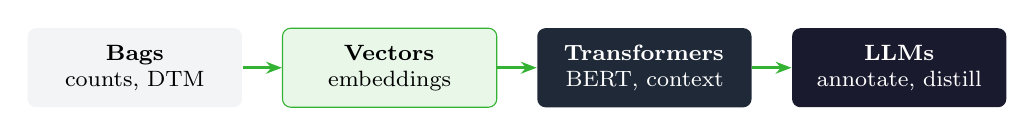
\begin{tikzpicture}[font=\footnotesize, node distance=0.5cm]
  \node[fill=lightgray, rounded corners=3pt, inner sep=6pt, text width=2.3cm, align=center] (d1)
    {\textbf{Bags}\\ counts, DTM};
  \node[fill=lightgreen, draw=wurgreen, rounded corners=3pt, inner sep=6pt, text width=2.3cm,
        align=center, right=0.5cm of d1] (d2)
    {\textbf{Vectors}\\ embeddings};
  \node[fill=bodytext, rounded corners=3pt, inner sep=6pt, text width=2.3cm, align=center,
        right=0.5cm of d2] (d3)
    {\textcolor{white}{\textbf{Transformers}}\\ \textcolor{white}{BERT, context}};
  \node[fill=darknavy, rounded corners=3pt, inner sep=6pt, text width=2.3cm, align=center,
        right=0.5cm of d3] (d4)
    {\textcolor{white}{\textbf{LLMs}}\\ \textcolor{white}{annotate, distill}};
  \draw[-{Stealth[length=2mm]}, wurgreen, line width=1pt] (d1) -- (d2);
  \draw[-{Stealth[length=2mm]}, wurgreen, line width=1pt] (d2) -- (d3);
  \draw[-{Stealth[length=2mm]}, wurgreen, line width=1pt] (d3) -- (d4);
\end{tikzpicture}
\end{center}

\medskip
{\small The newest tools do not make the older ones obsolete. A dictionary, a TF-IDF
classifier, a fine-tuned BERT, an LLM annotator --- each has its place. \textbf{The skill is
choosing well.}}

\medskip
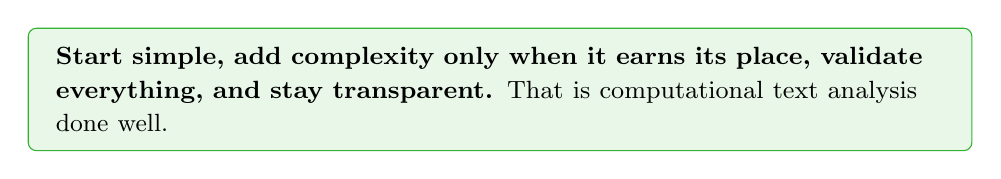
\begin{tikzpicture}
  \node[fill=lightgreen, draw=wurgreen, rounded corners=3pt,
        inner xsep=10pt, inner ysep=7pt, text width=\textwidth-24pt]{%
    {\small \textbf{Start simple, add complexity only when it earns its place, validate
    everything, and stay transparent.} That is computational text analysis done well.}};
\end{tikzpicture}
\end{frame}

% ── SLIDE 11: closing ─────────────────────────────────────────────────────
{
\setbeamertemplate{footline}{}
\begin{frame}[plain]
  \begin{tikzpicture}[remember picture, overlay]
    \fill[wurgreen] (current page.south west) rectangle (current page.north east);
    \fill[darknavy] (current page.south west) rectangle
      ([xshift=0.45cm]current page.north west);
    \node[text=white, font=\Huge\bfseries, anchor=west]
      at ([xshift=1.1cm, yshift=0.6cm]current page.west)
      {Thank you!};
    \node[text=darknavy, font=\normalsize, anchor=west, text width=11cm]
      at ([xshift=1.1cm, yshift=-0.9cm]current page.west)
      {From bags to vectors to transformers to LLMs --- you now have the full modern
       toolkit for computational text analysis.};
  \end{tikzpicture}
\end{frame}
}

\end{document}
